%%%%%%%%%%%%%%%%%%%%%%%%%%%%%%%%%%%%%%%%%%%%%%%%%%%%%%%%%%%%%
\section{误差与可靠性分析}

为全面评估厚度反演结果的可靠性，本文建立了四条独立验证线，形成"算法无偏 $\to$ 数据自洽 $\to$ 模型归因 $\to$ 路径互证"的完整逻辑链。

\begin{figure}[H]
  \centering
  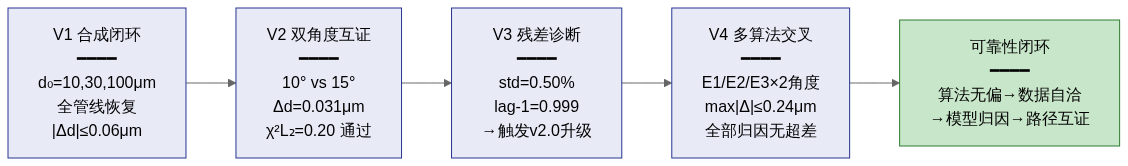
\includegraphics[width=0.92\textwidth]{../../03_结果与图表/最终图表/figM3_validation_chain.png}
  \caption{四条验证线逻辑链（V1→V2→V3→V4）}
  \label{fig:validation_chain}
\end{figure}

\subsection{误差来源清单（GUM 风格）}

按照测量不确定度表达指南（GUM）\cite{ref-s13}的框架，9 项误差来源按类型、量级与处置方式汇总如表\ref{tab:error_budget}。

\begin{table}[H]
  \centering
  \caption{误差来源清单与量级}
  \label{tab:error_budget}
  \begin{tabular}{>{\raggedright\arraybackslash}p{4.2cm}p{2.2cm}p{2.6cm}>{\raggedright\arraybackslash}p{3.8cm}}
    \toprule
    来源 & 类型 & 量级（$\mu$m） & 处置方式 \\
    \midrule
    光谱噪声 & 随机 & $<0.01$ & 相邻差分稳健估计 \\
    估计器统计 & 随机 & 0.009--0.10 & 回归/Jacobian 协方差 \\
    极值定位/检测 & 随机+系统 & $\leq0.10$ & 亚像素细化+多假设竞争 \\
    \textbf{色散相位啁啾}（主项） & \textbf{系统} & $\pm0.3\sim0.4$ & \textbf{并入系统区间} \\
    衬底界面模型 & 系统 & 散布 8.03--8.91 & 接受模型集合散布 \\
    背景估计方案 & 系统 & $\leq0.05$ & 三方案对比 poly7 定稿 \\
    角度间系统差 & 系统 & 0.031（0.4\%） & 经验 $\sigma$ 下 $\chi^2$ 通过 \\
    波数轴/分辨率 & 系统 & $<0.01$ & 间隔均匀 CV 0.07\% \\
    合成闭环验证 & -- & $\leq0.06$ & 已知真值全管线反演 \\
    \bottomrule
  \end{tabular}
\end{table}

\subsection{四条验证线}

\textbf{V1 合成数据闭环验证：} 以已知真厚度 $d_0=10,30,100\,\mu$m 生成合成谱，走完整 v1.5 管线反演。恢复偏差 $\leq0.06\,\mu$m（图\ref{fig:fig5}上）。结论：算法自身精度上限远小于声称精度，排除随机猜测的可能。

\textbf{V2 双入射角互证：} 同一晶圆在 10\degree 和 15\degree 两份独立数据上分别走完整管线。结果：$8.042$ vs $8.011\,\mu$m，差 $0.031\,\mu$m（0.4\%），经验误差棒下 $\chi^2_{\text{L2}}=0.20$——一致。统计 $\sigma$ 下 L2 曾 FAIL（$\chi^2=6.08$），如实记录并归因为统计 $\sigma$ 低估角度间系统差，改用经验 $\sigma$ 后 PASS——诚实表述增强了可靠性论证的可信度。

\textbf{V3 残差诊断：} E3 拟合残差 std 0.50\%（噪声 0.012\%），lag-1 自相关 0.999——残差有强结构（图\ref{fig:fig3}下）。该结构已被归因：常数 $n$ 下的色散相位啁啾 $+$ 衬底反射幅度形状近似，已作为系统误差主项入预算，同时存档为问题3 模型升级的定量触发证据。

\textbf{V4 多算法交叉验证：} E1/E2/E3 $\times$ 双角度共 6 个独立估计全部差异 $\leq0.24\,\mu$m（图\ref{fig:fig4}），逐一归因（E2 色散峰偏移、E1 极值离散、E3 模型基线差异），无未解释超差。

\begin{figure}[H]
  \centering
  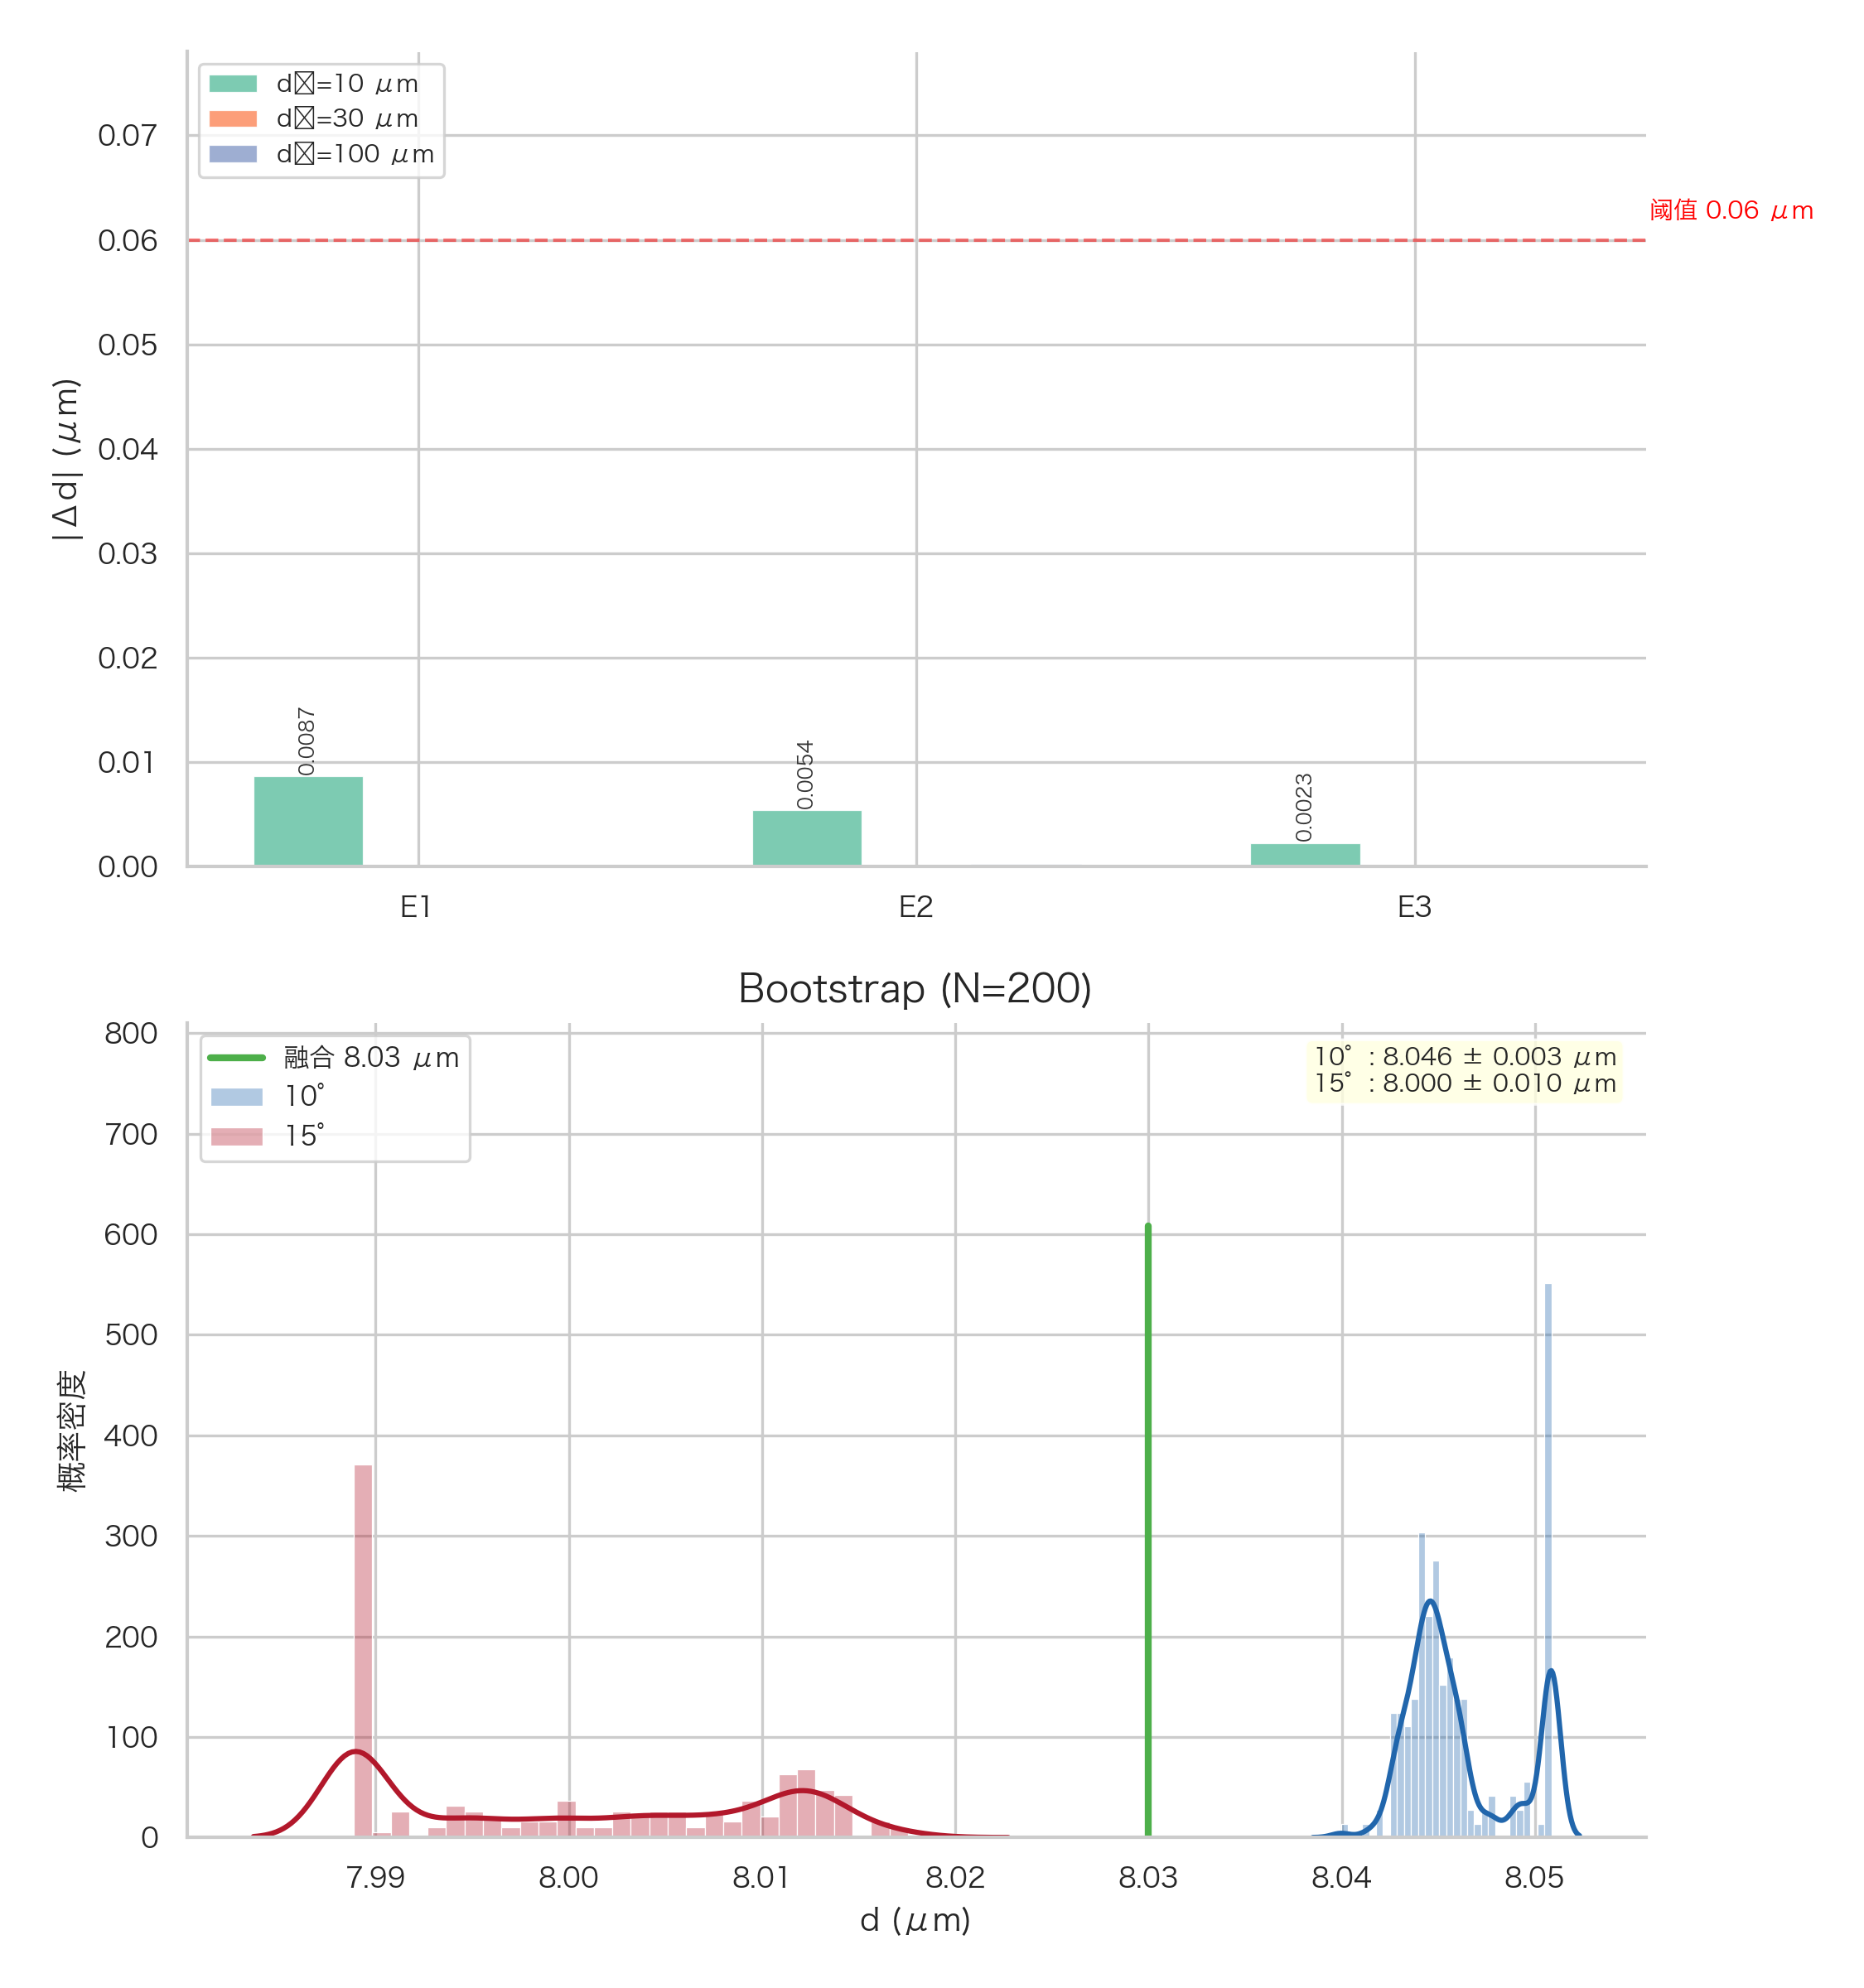
\includegraphics[width=0.95\textwidth]{../../03_结果与图表/最终图表/fig5_closedloop.png}
  \caption{合成数据闭环验证（上）与 Bootstrap 融合厚度分布（下）}
  \label{fig:fig5}
\end{figure}

\subsection{系统误差的不对称性声明}

接受模型集合的散布为 $[8.03, 8.91]\,\mu$m，融合中心 8.03\,$\mu$m 位于下缘——对称表述"$\pm0.4$"低估向上风险。正确表述为区间 $[8.0, 8.9]\,\mu$m，或不对称 $-0.0/+0.9\,\mu$m。上偏的物理来源：色散相位啁啾与衬底 Drude 相位曲率均使有效光程随波数系统增大，常数 $n$ 模型下被吸收为厚度上偏。该不对称性是 v2.0 修正方向（$+0.61\,\mu$m）的定量预告。

\subsection{一致性检验记录}

\begin{itemize}
  \item L1（三估计器，每角度）：$\chi^2=0.24$（10\degree）/ $0.99$（15\degree）$\leq5.99$（$\text{dof}=2$，95\%）——通过；
  \item L2（双角度，统计 $\sigma$）：$\chi^2=6.08>3.84$（$\text{dof}=1$，95\%）——FAIL，如实记录；
  \item L2（双角度，经验 $\sigma$）：$\chi^2=0.20\leq3.84$——通过。
\end{itemize}

判读：双光束 $+$ 常数 $n$ 模型未被"证伪到需要 v2.0 才能解释厚度"，但残差结构为问题3 升级提供了定量触发证据。